% Chapter 2

\chapter{Background and Theory} % Main chapter title

\label{Chapter2} % For referencing the chapter elsewhere, use \ref{Chapter2} 

%----------------------------------------------------------------------------------------


\section{Sound Propagation}

In order to study the concept behind acoustic contrast control we first need to understand how the sound propagates from the speakers to the control points. The theoretical model that sets the stage is the Green's function. This function models the propagation of a soundwave of a system through a linear differential equation. Being an ideal model, it is a good approximation only in certain scenarios, this is because it can only describe a soundwave using a spherical field. This, while true at lower frequencies, it's not the real behavior of a wave once reached a certain critical frequency. What happens is that the propagation pattern is not spherical anymore, but start becoming multi-lobed, this particular shape is called cardioid. In the following figure we can see an example of this phenomenon. The propagation pattern (and the critical frequency) varies wildly between different loudspeaker models, the figure shows the behavior of a specific model, nevertheless, it can give the reader an idea on how the sound at different frequencies can propagate from a speaker.

\begin{figure}[th]
\centering
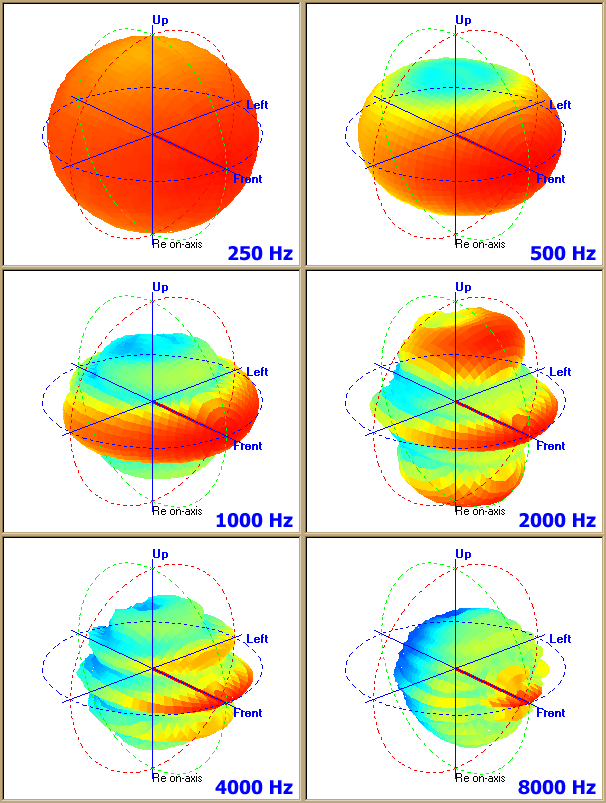
\includegraphics[width=8cm,height=9cm,keepaspectratio]{Figures/directivity}
\decoRule
\caption[Propagation pattern]{Propagation pattern of a loudspeaker at various frequencies. The speaker model is a Bosch 36 watt LA1-UW36-x. The figure is taken from on-line resources.}
\label{fig:directivity}
\end{figure}

We will use the Green's function for the very first part of the implementation of the acoustic contrast control algorithm, when testing it in a simulated scenario.

\subsection{Green's function}{}
\label{subsec:greenfct}

Resolving the sound propagation problem can be reduced to finding the appropriate weights to a matrix that correlates the wave origin points with the detection points. An easy and widespread way of solving the problem in the literature is by using the Green's function \parencite{elliott_robustness_2012,kuttruff_room_2014,shin_maximization_2010}.
\\
This function proposes a solution to a system of non-homogeneous differential equations. By finding the solution to said system it is possible to correlate the acoustic energy detected in a certain point in space with a linear combination of origin point sources. This relationship is linearly dependent from the distance of said point from the individual sound sources, multiplied the air resistivity.
\\
\\
Let's give an operative definition of the Green function by expressing the easiest boundary value problem for a differential operator, by saying

\[ L u = f,\quad u(a)=u(b)=0 \]

(it is reminded to the reader that since we're talking about a differential equation here $f$ is a function and $u(a), u(b)$ are boundary values), where $L = \frac{-d^2}{dx^2}$ is the second order derivative operator, in this case the Green function can be expressed by using $ - G'' = \delta (x - \xi)$, resolving $u$ then becomes equal to finding

\[ u=\int_{a}^{b} G(x,\xi)f(\xi)d\xi\]
where $f(\xi)$ is the value of the function in the point 
$ a \le \xi \le b $, and
\\
$G(x,\xi) = - \rho(x - \xi) + Ax + B$ is the Green's function, the result of the integration of $-G''$, $\rho$ is the ramp function ( the ramp function is the double integral of the delta function).
\\
\\
This means that it is possible to calculate the value that a differential equation takes in a certain point by knowing its input, the propagation function and some boundary values, this is conceptually not dissimilar of solving a linear system $Ax=y$, where instead of linear equation we have differential equations.
\\
Expanding on this concept it is possible to define a system of differential equations, where instead of a single source point it possible to calculate the effect that a linear combination of sources have in a determined point (in other words, the solution of the system).
\\
\\
This is very significant, because by knowing the Green's function (which is our theoretical model) of a soundwave, we can correlate the effect (having some acoustic energy in a point in space) with having a cause (a single, or even multiple sound sources, by the principle of superposition) and viceversa, that is, knowing how much does a source effect the total energy figure in a destination point.
\\
\\
The Green equation for a sound field is \parencite{elliott_robustness_2012,kuttruff_room_2014,shin_maximization_2010}:

\begin{equation}
G(r)=-j \rho 2 \pi f \frac{e^{-j k r}}{4 \pi r};
\label{eqn:green}
\end{equation}

Where $j$ is the imaginary unit, $\rho$ is the atmospheric air density. $\rho = 1.21$ is the air density value at sea level and at $15^{\circ}$C, $k$ is called the wave number and is equal to $k = \frac{2 \pi}{\lambda}$ with $\lambda$ as the wavelength and $r$ is the distance (radius) between source and destination. 
\\
\\
Unfortunately the solution of the Green's function exist in closed form only in some simple cases. In order to determine how a soundwave propagates in a more complex space (such the one of an anechoic chamber or a listening room) it is necessary to directly measure the output of a speaker and correlate it with the input used as solicitation.
\\
One more problem to consider is the one regarding the assumption of having a spherical propagation pattern. Unfortunately this kind of behavior is true for soundwaves having a relatively low frequency, in fact, by increasing the sound frequency the real world scenario grows more distant to the ideal one, the spherical pattern tends to resemble a multi-lobed one. The critical frequency, shape and number of the lobes depend on the dimensions, power, construction material, shape of the speaker cone and can be described only on a case by case basis.


\section{Sound generation and harmonics}
\label{sec:soundgen}

The sound actuator, or loudspeaker, is an electromagnetic device that uses a rapidly changing electrical bipole, generated by a coil glued on a cone-shaped cloth or silicate, usually made of copper, to generate movement through the interaction of the resulting magnetic field (as described by the Ampere-Maxwell laws), with a permanent or semi-permanent magnet situated behind the moving coil.
\\
\begin{figure}[th]
\centering
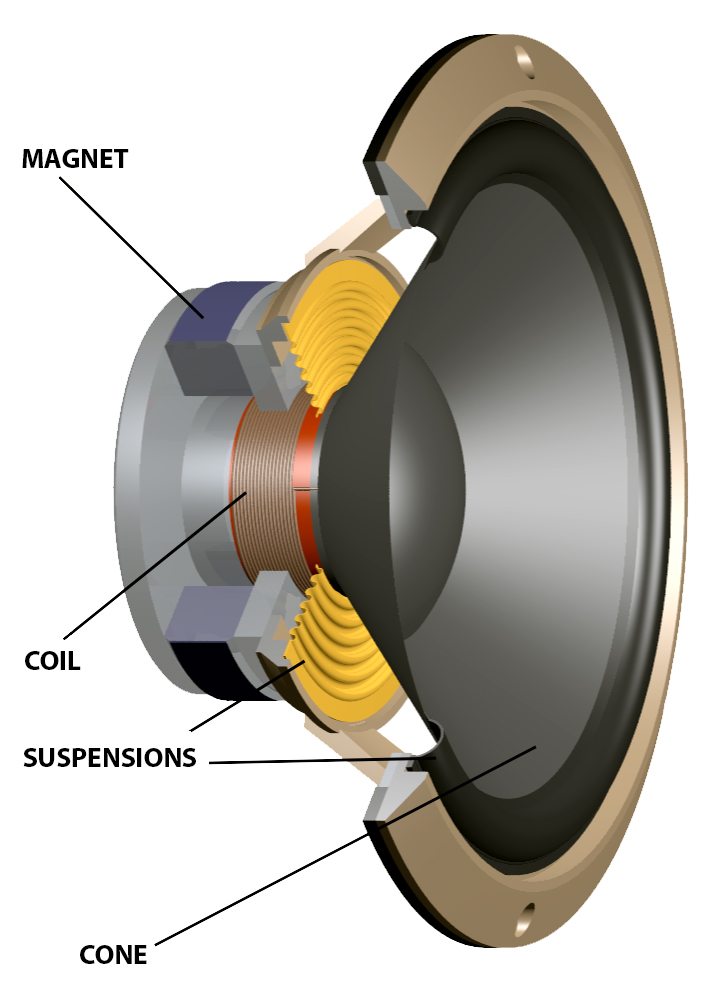
\includegraphics[width=7cm,height=7cm,keepaspectratio]{Figures/loudspeaker}
\decoRule
\caption[Loudspeaker representation]{Cut-out of a generic loudspeaker, here the reader can recognize the main elements. The figure is taken from on-line resources and modified.}
\label{fig:loudspeaker}
\end{figure}

The kind of behavior that a loudspeaker shows changes at low and high amplitudes. This dependency from the amplitude is non linear. As a consequence of this nonlinearity we have that in response to a stimuli signal, some frequency components, non existent in the input, will appear. This components will show themselves at integer multiples of the input frequency, for instance, if the input is a $200$Hz sine-wave with a certain amplitude, in the frequency response of the system, some peaks (usually, but not always, with a smaller amplitude than the first one) will appear at $400$Hz, $600$Hz and so on. These components are called higher order harmonics.

\begin{figure}[th]
\centering
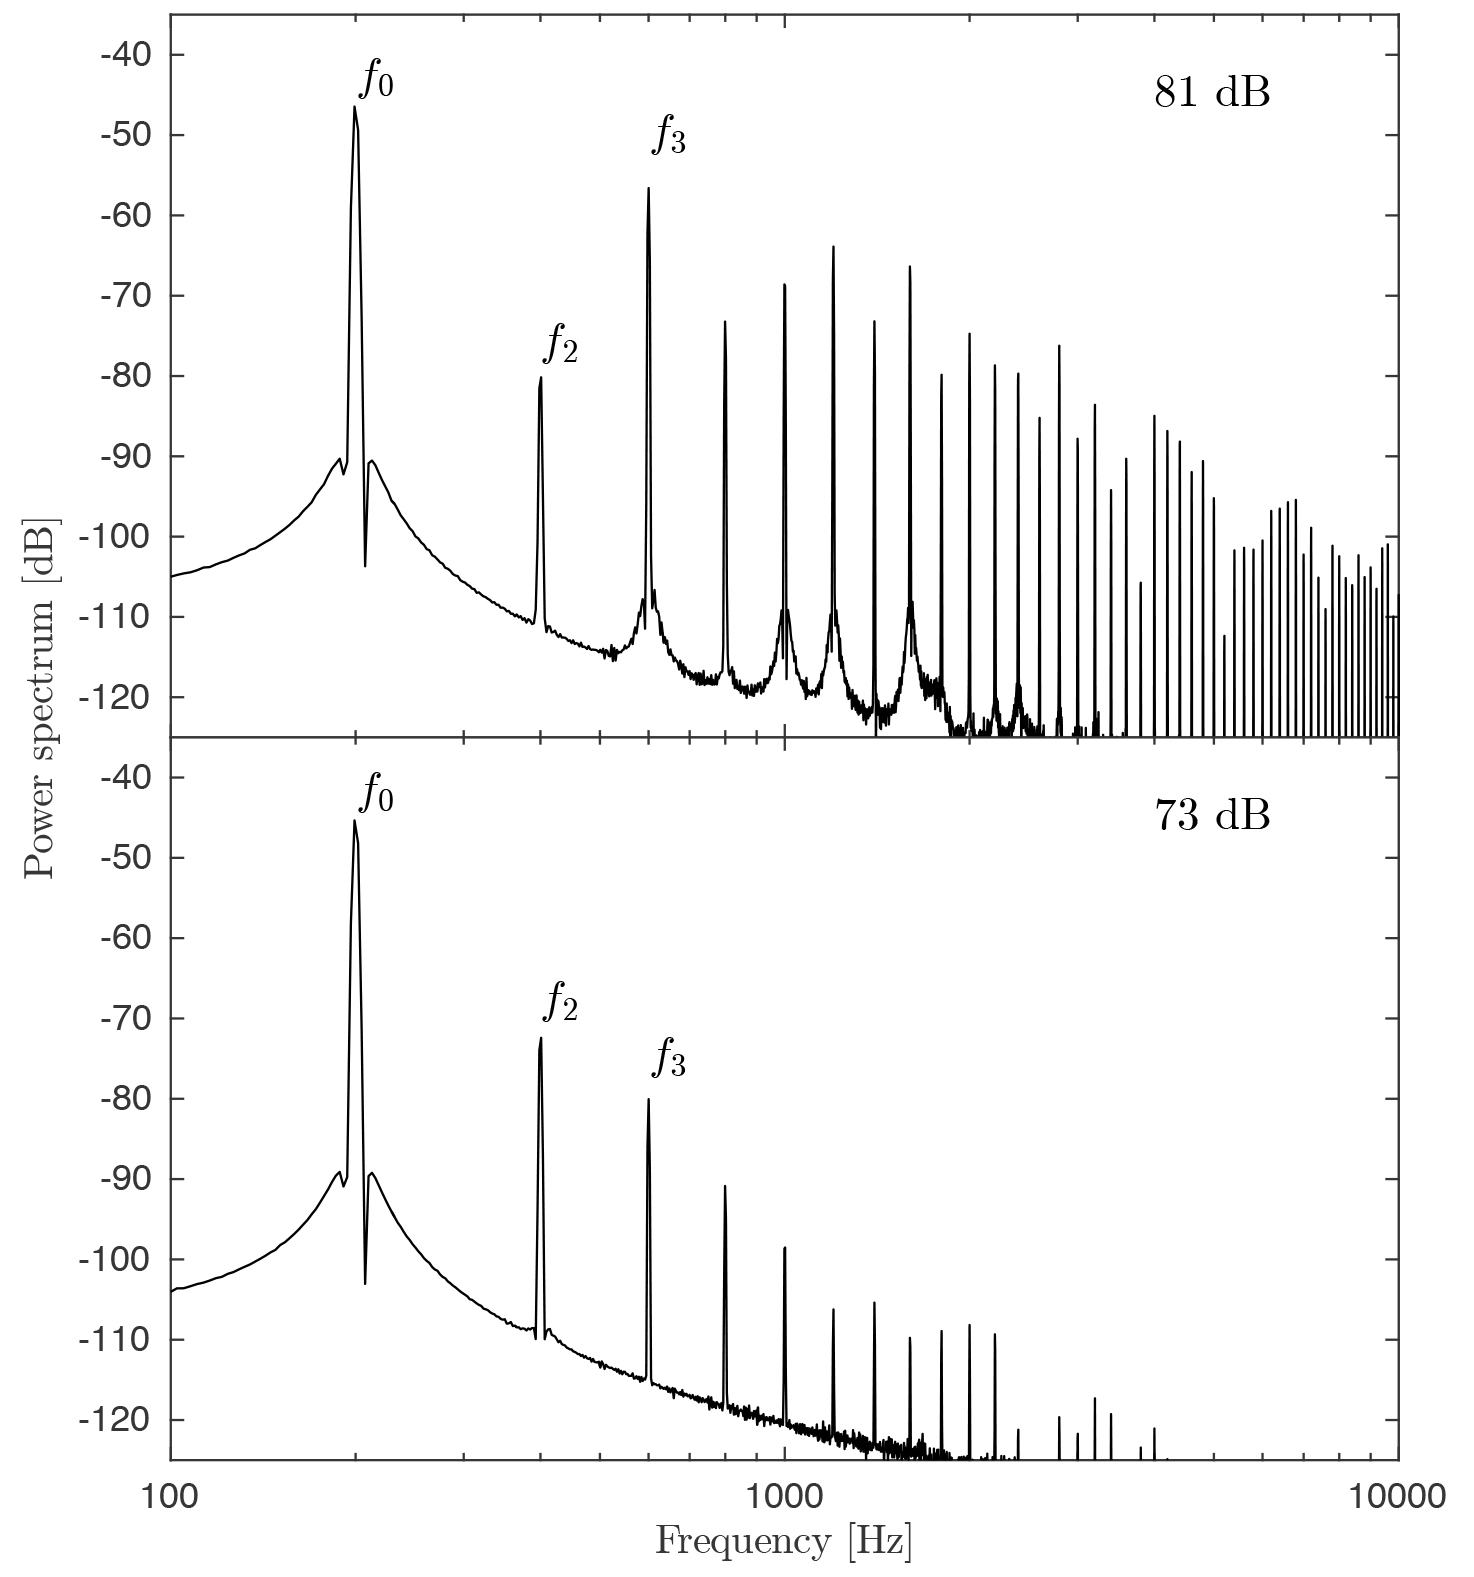
\includegraphics[width=9cm,height=10cm,keepaspectratio]{Figures/nonlinearities}
\decoRule
\caption[Frequency response of a loudspeaker emitting a sine wave at 200Hz]{Frequency response of a loudspeaker emitting a sine wave at 200Hz. The reader can notice the higher order harmonics at multiples of $200$Hz. Increasing the amplitude increases the presence of nonlinearities. Graph taken from \parencite{ma_personal_2016}.}
\label{fig:nonlinearities}
\end{figure}
We can also see from the figure that playing at high amplitudes generates even more non linearities, this is because the cone displacement increases, so the force applied on the coil varies more \parencite{ma_personal_2016}.
\\
\\
Additionally, if the input signal has significant components at more than one single frequency, these will interfere with each other, generating a phenomenon known as inter-modulation distortion, the interaction between these components will form additional signals at frequencies that are not just at integer multiples of said components, but also at the sum and difference frequencies of the original ones. This generates a cascade of unwanted components that interact with each other and generally degrade the signal-to-noise ratio of the system.
\\
\\
The nonlinear behavior showed by a loudspeaker at low amplitudes is given by the fact that the stiffness of the cone is not constant for varying amount of force exerted, this means that the displacement is different from the one intended, in other words the mechanical characteristics of the component (mainly the cone) constituting the speaker deviate from the expected behavior.
\\
High amplitudes tend to accentuate the imperfections in the driver unit, for instance, local changes in the rigidity of the cone, or misplacement of the glue that holds the cone to the frame. Moreover, the displacement in the two directions (front/back) is not equal, mainly because the mechanical impedance is not equal in the two directions. Also, the force that couples the mechanical and electrical side of the speaker is not constant. We can describe this force as the integral of the magnetic flux density $B$, versus voice coil wire length $l$. We can plot the force factor $Bl(x)$ and see that it is not a constant, but it depends on the displacement $x$ of the coil. More distant is the coil from the magnet, less force it will experience \parencite{klippel_tutorial:_2006}.

\begin{figure}[th]
\centering
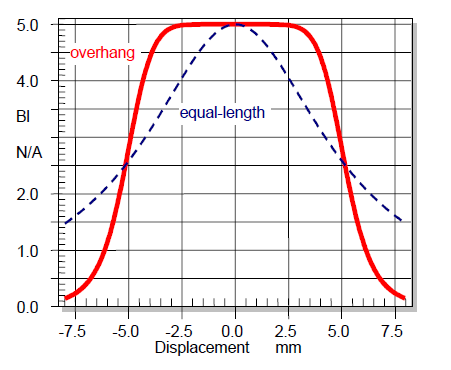
\includegraphics[width=8cm,height=8cm,keepaspectratio]{Figures/displacement}
\decoRule
\caption[Force factor vs. displacement]{Plot of the force experienced by the coil versus its displacement. Overhanging is a method to improve the performances, it consists in making length $l$ of the coil bigger than the section of the magnet, so that the magnetic flux is less dependent from the relative position of the cone. Graph taken from \parencite{klippel_tutorial:_2006}.}
%\label{fig:directivity}
\end{figure}

At low frequencies the main cause of nonlinearity is the big excursion of the coil. This causes a big variation in the magnetic field, which exerts a smaller force when the coil is distant from the magnet.
\\
At high frequencies, the rapid movement of the cone strains the materials, that start showing different properties from the expected ones, these phenomena are known as break-up modes. At higher frequencies the cone starts to bend, instead of moving as a whole generating resonance effects, this happens at fixed frequencies that are not related to the input signal.
\\
\\
As we've just discussed, a speaker shows nonlinear behavior when excited in ranges close to its operational limits. The intensity of the nonlinearities generated is not the same for all of these critical modes. As already seen in figure \ref{fig:nonlinearities}, the worst scenario is when the speaker is excited at high amplitudes and low frequencies.
\\
\\
The presence of nonlinearities is detrimental to the performance of the acoustic contrast filter we will calculate, since it reduces the contrast figure achievable, this is because of two reasons.
\\
First, as previously stated, the distortions are parts of the output signal that weren't present in the original one, they act essentially as noise, therefore compromise the contrast figure.
\\
Second, the model used in the algorithms that implement the ACC method only treats the linear part of the system. In principle it is possible to define a more complex model that takes into account the higher harmonics, but developing such a model is beyond the scope of this project. Even though this is a big issue of the current control methods available, this problem has been avoided during this work, by choosing an appropriate frequency range and playing at low enough amplitudes, so that their generation is not too evident.

\section{Acoustic Contrast Control}
\label{sec:acc}

The first description of an Acoustic Contrast Control (ACC) algorithm was given in 2002 \parencite{choi_generation_2002}. Since then, different contributors in the academia have proposed new solutions that refine the concept \parencite{elliott_robustness_2012,cai_time-domain_2014}, in this section we will discuss the principles that guide these algorithms and some important aspects that have been considered for choosing the appropriate one for this thesis work.
\\
\\
The main principle of ACC is to reproduce a soundwave that has the same intensity (amplitude) and opposite phase with respect with another soundwave that we do not wish to have. When these waves meet they cancel each other out. This is intuitively simple to understand, since the propagation of a soundwave can be expressed as a portion of space where air particles get compressed or expanded as the wave passes by, the amount of compression (or expansion) depends on the intensity of the wave, the kind of adiabatic transformation (compression or expansion) depends on its phase and the direction depends on the position of the source. If two equally ample, but opposite fluxes of air meet with exactly the opposite phase, they will destructively interfere with each other. For the same reason, two fluxes with the same phase will add to each other, and every result in between this two cases will lead to an increase or decrease of the resulting flux, depending on the relative phase difference of the two waves.
\\
\\
This simple principle has led to the development of active noise control (ANC), a control method that is relatively widespread that appears in many consumer-grade electronics, especially headphones and earplug.
\\
ACC is fundamentally different than ANC. While the implementation of ANC can be relatively inexpensive, mostly because the signal and the noise are well distinct (in principle, everything coming from the external world is treated as noise), and since the sound sources are close the ear canal of the user the power required to cancel the undesired sources is very limited. With ACC instead, two signals can coexist in the same space, and there is no clear distinction between what is the signal and what is the noise by itself, but those term acquire now a local significance, meaning that a particular sound might be considered noise only in a limited region of space. The fact that more sounds have to share the same channel introduces a new set of constraints, for instance, adding acoustical energy to the environment (by increasing the control effort) is not necessarily the best course of actions to increase the contrast figure.
\\
As explained in section \ref{sec:soundgen}, high amplitude sounds generate higher harmonics that are very difficult to control, sound propagation pattern diverges from the spherical formulation described by subsection \ref{subsec:greenfct} and also the room acoustics now become a factor to consider when designing the algorithms. Tackling these issues has required 15 years of research and many more years will probably be necessary before seeing the adoption of this technologies by the industry for mainstream consumer market.
\\
\\
Going back to the specifics of the ACC, it is conceptually equivalent to have two different sound signals that have to be addressed to two different zones, or having a single signal that has to be reproduced in a zone, while suppressed in another one. In all sections of this work, the second case will be the one treated.
\\
\\
Let's now give a mathematical definition to ACC, let's start by defining the acoustic energy $e_b$.
\\
For a volume $V_b$, the acoustic energy is defined as

\begin{equation}
e_b=\frac{1}{V_b}\int_{V_b}p(\vec{x}) p(\vec{x}) dV
\label{eqn:acousticenergy}
\end{equation}

please note that $b$ refers to the bright zone, the formulation for the dark zone is identical. $p(\vec{x})$ is the sound pressure, that can be expressed \parencite{choi_generation_2002} as

\begin{equation}
p(\vec{x})=\sum\limits_{i=1}^K \textit{G}(\vec{x}|\vec{x}_c^{(i)})q_c(\vec{x}_c^{(i)}) = G(\vec{x}|\vec{x}_c)q_c
\label{eqn:soundpressure}
\end{equation}

where $K$ is the total number of sources available, $\textit{G}(\vec{x}|\vec{x}_c^{(i)})$ is the propagation function (the Green's function described in section~\ref{subsec:greenfct}) between the position $\vec{x}$ and the control source position $\vec{x}_c^{(i)}$ of loudspeaker $i$ (where $i=1...K$) and $q_c$ is the volume velocity, which measures the amount of air flowing in a given volume, per unit of time.
\\
\\
The energy can also be expressed by calculating the square of the complex magnitude of the pressure

\begin{equation}
\label{eqn:energycorrelationformulation}
\vec{e_b}=\frac{1}{V_b}\int_{V_b}p(\vec{x}) * p(\vec{x}) dV = q_c^H\left(\frac{1}{V_b}\int_{V_b} \textit{G}^H(\vec{x}|\vec{x}_c)\textit{G}(\vec{x}|\vec{x}_c) dV\right)q_c = q_c^H R_b q_c
\end{equation}

where $R_b$ represents the spatial correlation of the pressure field in the bright zone produced by each control source \parencite{choi_generation_2002}.
This will prove especially useful later, because, while the propagation (Green's) function cannot be expressed in a real experimental scenario, it's relatively easy to calculate the correlation figure, in particular, the acoustic contrast can be defined \parencite{cai_design_2013}, as the ratio of

\begin{equation}
\delta=\frac{e_b}{e_d}=\frac{w^T R_b w}{w^T R_d w}
\label{eqn:contrast}
\end{equation}

Where $w$ is a set of weights derived from the ACC algorithm explained below, while $R_b(n), R_d(n)$ refer to the $n$th control point, either in the bright or dark zone. This spacial dependence is implicit in defining the correlation, therefore omitted from this point forward.
\\
It appears clear that the maximization of such ratio can be achieved in two ways: maximizing the energy in the bright zone, or maximizing the ratio between total energy and energy in the bright zone. In both cases, finding the optimum set of weights, corresponds to find the solution to a Lagrange optimization problem.
\\
\\
Let's consider the first case, the output power can be written as a function of the volume velocity as $J_0=q_c^H q_c$ \parencite{choi_generation_2002}, the problem can now be formulated as constrained optimization problem under the form
\\
\[ \begin{aligned}
&\text{maximize} \quad
&& e_b=q_c^H R_b q_c
&\\
&\text{subject to} \quad 
&& J_0=q_c^H q_c
\end{aligned} \]
\\
which, introducing the Lagrange multiplier $\alpha$ can be written in a single equation as
\[\begin{aligned}
&\text{maximize} \quad J=q_c^H R_b q_c + \alpha(J_0-q_c^Hq_c)
\end{aligned}\]

taking the partial derivatives $\frac{\delta}{\delta q_c}$ and $\frac{\delta}{\delta \alpha}$ and solving the resulting system for $\alpha$ \parencite{choi_generation_2002,elliott_robustness_2012}, we get

\begin{equation}
\label{eqn:alpha}
\alpha=\frac{e_b}{J_0}=\frac{q_c^H R_b q_c}{q_c^Hq_c}
\end{equation}
\\
The acoustic contrast is maximized when the volume velocity $q_c$ is highest. Finding this maximum value is equivalent to find the solution to the generalized eigenvalue problem written as $\lambda q_c=A q_c$; $q_c$ can be treated as an eigenvector that has its maximum when it's equal to the maximum eigenvalue of $R_b$. The solution can be written as $q_{max} = \frac{\sqrt[]{J_0}}{\alpha} R_b^H$. In simpler terms, when the correlation, times a function that somehow describes the characteristics of the channel, is maximized, we have the maximum acoustic contrast
\parencite{shin_maximization_2010,choi_generation_2002}.
\\
\\
This formulation is not the most convenient one, because, while we maximize the energy in the bright zone, it doesn't take into account the energy that is being outputted in the dark zone, this can generate a relatively "loud" area, even in the dark zone. Moreover, as already explained, outputting higher powers generates non linearities in the speakers, which is highly undesirable, since it can further reduce the contrast, and more generally, create sound artifacts that impact negatively on the user experience. There is also a physical limit on the maximum power achievable given by the specific hardware (amplifiers, loudspeakers) that are being used.
\\
\\
The second method takes into account the enrgy in both zones and tries to maximize the contrast by tuning the output energy making sure that a minimum amount "leaks" into the dark zone. The Lagrange parameter adds flexibility to the algorithm, meaning that having a large $\alpha$ generates more energy in the bright zone. The increase in sound intensity in this zone is more beneficial (gives more contrast) than keeping a lower energy level, vice versa, a smaller $\alpha$ means that in order to get the best result is best to limit the output power. 
\\
The optimization function can be written as
\begin{equation}
\label{eqn:beta}
\beta=\frac{e_b}{e_t}=\frac{q_c^H R_b q_c}{q_c^H R_t q_c}, \quad e_t = e_b + e_d, \quad R_t = R_b + R_d
\end{equation}
\\
The cost function can be calculated in the same manner
as the maximization method, the maximum is obtained from the eigenvector of $R_t^{-1} R_b = \beta_{max}$ corresponding to the largest eigenvalue of the matrix \parencite{choi_generation_2002,schellekens_time_2016}. This, once convolved with the output signal, will generate acoustic contrast.
\\
Both the approaches discussed above are frequency dependent, meaning that a control frequency is defined in the algorithm and the optimization problem is then applied to it.
\\
\\
Looking closely at the equations \ref{eqn:beta} and its solution, it is possible to notice a fundamental problem, first treated by \parencite{elliott_robustness_2012}, that is, sometimes there can be numerical problems related to the correlation matrices, equation \ref{eqn:energycorrelationformulation} says that $R_b =\textit{G}^H(\vec{x}|\vec{x}_c)\textit{G}(\vec{x}|\vec{x}_c)$, in order to be invertible, has to be full rank. It might happen that $R_t$ is singular, or non-invertible (remember that $ R_t = R_b + R_d$).
\\
\parencite{elliott_robustness_2012} introduced a regularization term to improve on the robustness of the algorithm. The problem with having a frequency domain formulation is that the response of the filter is controlled only at determined frequencies, in particular, these algorithm chooses a control frequency (the one that leads to the maximum contrast) and increase its output power. This can lead to wild variations of the response at non-control frequencies and, in general a noticeable distortion of the FR in the bright zone.
\\
\\
In order to solve this controllability problem, \parencite{cai_time-domain_2014} have created two methods that provide contrast, while controlling the frequency response in the bright zone, in a broad range of frequencies. These methods are called Broadband Acoustic Contrast Control Response Variation (BACC-RV) and its later variation, Broadband Acoustic Contrast Control Response Differential (BACC-RD).
\\
These method have a fundamental difference with regard of the ones just described (though they have a similar formulation). That is, both are time domain resolved.
\\
All the frequency domain filters have to be brought in the time domain before being applied to the output sound signal (using the Inverse Fourier Transform). Moreover, in order to have a good frequency response, only a long filter can provide a good contrast over a broad spectrum of frequencies, condition that is not as fundamental in the time domain (even though in principle a longer filter it's always preferable, since it improves the contrast). This causes an unnecessary delay given by the domain conversion. Instead of measuring the frequency response and define a control frequency it is possible instead to work directly with the impulse response of the system.
\\
\\
Now that the reader has been given an overview of ACC fundamentals, it will appear more clear why BACC-RV/RD have been the method considered for the development of the core algorithms of this work, and the starting point for the modifications proposed in later sections (Chapter \ref{Chapter4}). The RD method has been preferred over the RV one because, even though it has very similar performances \parencite{cai_time-domain_2014,schellekens_time_2016}, it only has 2 tuning parameters instead of 3.
\\
\\
The formulation of the eigenvalue problem for the BACC-RD algorithm, solved using the Lagrange multipliers problem is expressed as

\begin{equation}
L = \frac{w^T R_b w}{\beta w^T R_d w + (1 - \beta) RD + \delta w^T w}
\label{eqn:lagrange}
\end{equation}
Where $\beta$ is a weight factor, setting the trade-off between the acoustic contrast and the flatness of the frequency response in the bright zone in the frequency range of interest, $0\le \beta \le 1$. $\delta$ is the regularization term, introduced by \parencite{elliott_robustness_2012}, it ensures robustness against statistical outliers in the noise figure, defining a maximum deviation that is allowed in the correlation to its mean square value. $R_b, R_d$ are the correlation matrices in the bright and dark zones and $w$ is a vector of weights, which maximization will eventually generate the contrast.
\\
\\
The optimum of the equation is deducted by maximizing $w$, it can be formulated by the expression
\\
\begin{equation}
w_{BACC} = \underset{w}{\operatorname{argmax}} \; L
\label{eqn:optimization}
\end{equation}

the solution of equation \ref{eqn:optimization} returns the BACC filter which generates the highest acoustic contrast. This is term corresponds to the largest eigenvalue of the matrix
\\
\begin{equation}
\delta=\frac{e_b}{e_d}=\frac{w^T R_b w}{w^T R_d w}
\label{eqn:contrast}
\end{equation}\[ \left[ \beta RD + \frac{1 - \beta}{(J-1) K}\sum\limits_{k=1}^{K} \Re \{ (V S_k)^H (V S_k) \} + \delta U \right]^{-1} R_b\]
\\
Where $U$ is the identity matrix \parencite{cai_time-domain_2014}, $K$ is the number of control points available, which is where the microphones will be positioned for the experiments, $J$ is the number of control frequencies and $V$ and $S_k$ are two matrices, defined as

\[V=\begin{bmatrix}
    -1 & 1 & 0 & \dots & 0 & 0 \\
    0 & -1 & 1 & \dots & 0 & 0 \\
    \vdots & \vdots & \vdots & \ddots & \vdots \\
    0 & 0 & 0 & \dots & -1 & 1
	\end{bmatrix}, \quad
S_k= \begin{bmatrix}
    s_{k}^T(f_1) \\
    \vdots \\
    s_{k}^T(f_j)\\
    \vdots \\
    s_{k}^T(f_J)
	\end{bmatrix}
\]
The product $V S_k$ controls the points where the frequency response is optimized, which total number of these frequencies is $J$. $S_k$ is in reality $S_{bk}$ or $S_{dk}$, depending on which zone we are considering.
\\
The $V$ matrix effectively perform the differentiation of each of the $k$ output vectors $s_{k}(f)$. The control frequencies $f_j$ are the points where the contrast between the two zones will be maximized. The number of control points depends on the on the sampling frequency of the signal, while the space between them is affected by the length (in samples) of the filter. A longer filter allows for more closely spaced control frequencies (also called bins), this will increase the contrast figure.
\\
At first glance one can see that equation \ref{eqn:lagrange} is similar to the formulation \ref{eqn:contrast}, with the addition of the $RD$ term and two parameters, $\beta,\delta$ \parencite{cai_time-domain_2014}.
\\
The $RD$ term is described by

\begin{equation}
RD = \frac{1}{(J-1)K}\sum\limits_{k=1}^K (V S_k w)^H (V S_k w)
\label{eqn:RD}
\end{equation}
\\
The $S_k$ matrix is derived by Fourier transforming the output vector, which is the convolution between input signal, room impulse response and the filter vector $w$, assuming the input signal is a Dirac's delta function, it can also be written as (with the bright zone formulation)

\[S_{bk}=\mathcal{F}[y_{bk}(n)]=\mathcal{F}[w^T r_{bk}(n)]\]
\\
which is the product between the weight vector and the filtered impulse response of the system to the Dirac's delta, as generated by source point $k$ \parencite{cai_time-domain_2014}.
\\
The filtered vector $r_{bk}(n)$ is equal to

\[ r_{bk}(n) = [h_{b_1k}(n),\dots,h_{b_1k}(n-M+1),\dots\dots, h_{b_Lk}(n),\dots,h_{b_Lk}(n-M+1)]^T\]
\\
As we can see, it filters the impulse response between the source $l$ and the control point $k$ and has length $M$. 
The $b$ in the notation specifies that the control point is in the bright zone. The equivalent equation for the output vector $y_{dk}$ is described in the same way.
\\
\\
In the case the signal is wideband, we might wonder how the filtered vector can be described. The optimized frequency response $\rho_{bk}(f)$  can be written as

\begin{equation}
\rho_{bk}(f) = \sum\limits_{n=0}^{M+I-2} y_{bk}(n) e^{-j2\pi f n T_s}=w^T s_{bk}(f)=w^T [r_{bk}(n) e^{-j2\pi f n T_s}]
\label{eqn:freqresp}
\end{equation}

$y_{bk}$ is the output vector, also called the global response, it comprises the input, the filter weights $w$ and the room transfer function $h_{blk}$ between the loudspeaker $l$ and the control point $k$. It has length $M+I-1$.
$M$ and $I$ are the lengths of the weights vector and the system's impulse response (in the time domain). These values can be adjusted independently of each other. As we can see from this formulation, the control frequencies vector $S_k$ is multiplied with $w^T$, which weights the contribution that each frequency bin has to the (wideband) frequency response of the system. The spacing between bins depends on the length $M$ of the filter, a longer filter can more finely control the frequency response of the system.
\\
\\
The $RD$ term can be expressed in terms of the frequency response \parencite{cai_time-domain_2014,schellekens_time_2016}, with a formulation similar to the one of the mean square error

\begin{equation}
RD = \frac{1}{(J-1) K} \sum\limits_{k=1}^{K} \sum\limits_{j=1}^{J-1} |\rho_{bk}(f_{j+1}) - \rho_{bk}(f_j)|^2
\label{eqn:RDfreqresp}
\end{equation}

The smaller is this term, the flatter frequency response we will be able to achieve.

For consistency with equation~\ref{eqn:acousticenergy}, it can be said that \parencite{cai_time-domain_2014}
\[ y_{bk}(n)=w^T r_{bk}(n), \quad e_b=\sum\limits_{k=1}^{K}\sum\limits_{n=0}^{M+I-2}\frac{y_{bk}^2(n)}{K} = w^T R_b w\]
\\
As previously stated, an interesting property of the algorithm is that we have two parameters, $M$ and $I$, those are, respectively the IR length and the FIR filter length, we can arbitrarily decide to cut short the time-domain response of the room. This characteristic will prove extremely useful for the management of the computational resources available, since it will dramatically speed up the calculation of the $R_b$ and $R_d$ matrices.
\\
Moreover, having an adjustable filter length makes this kind of filter effective even at short lengths. Of course, the longer the impulse response of the system, the more we will be able to control the system. As we will see later, this also means increasing the number of operations necessary to calculate the filter, specifically, the correlation matrices $R_b, R_d$ increase with the square of the filter length, this for each microphone-speaker pair. As we will see in chapter ~\ref{Chapter4} this makes filters longer that 600 taps very impractical to calculate.

